\section{Конструкторская часть}

В этом разделе будут представлены схемы и/или псевдокоды реализуемых алгоритмов.

\subsection{Требования к ПО}
К программе предъявляется ряд требований:
\begin{itemize}[]
	\item искомая подстрока имеет размер $S$ от 6 до 10 символов;
	\item при генерации исходной строки шанс 7/8 сгенерировать подстроку из $S$ случайных символов;
	\item при генерации исходной строки шанс 1/8 сгенерировать искомую подстроку;
	\item на вход подается строка и искомая в ней подстрока;
	\item на выходе требуется получить файл с записями индексов вхождения подстроки.
\end{itemize}

\newpage
\subsection{Разработка алгоритмов}

В листинге~\ref{alg:standart} рассмотрен псевдокод стандартного алгоритма поиска подстроки в строке.

\begin{algorithm}[H]
	\caption{Стандартный алгоритм}
	\label{alg:standart}
	\SetAlgoLined
	\KwIn{Строка $text$, подстрока $pattern$}
	\KwOut{Индекс первого вхождения $pattern$ в $text$, или -1 если не найден}
	$n \gets \text{length}(text)$\;
	$m \gets \text{length}(pattern)$\;
	\For{$i \gets 1$ \KwTo $n - m + 1$}{
		$j \gets 1$\;
		\While{$j \leq m$ \textbf{and} $text[i + j - 1] = pattern[j]$}{
			$j \gets j + 1$\;
		}
		\If{$j > m$}{
			\KwRet{$i$}\;
		}
	}
	\KwRet{-1}\;
\end{algorithm}

\newpage

На рисунке~\ref{fig:linear} приведена последовательная реализация программы.

\begin{figure}
	\centering
	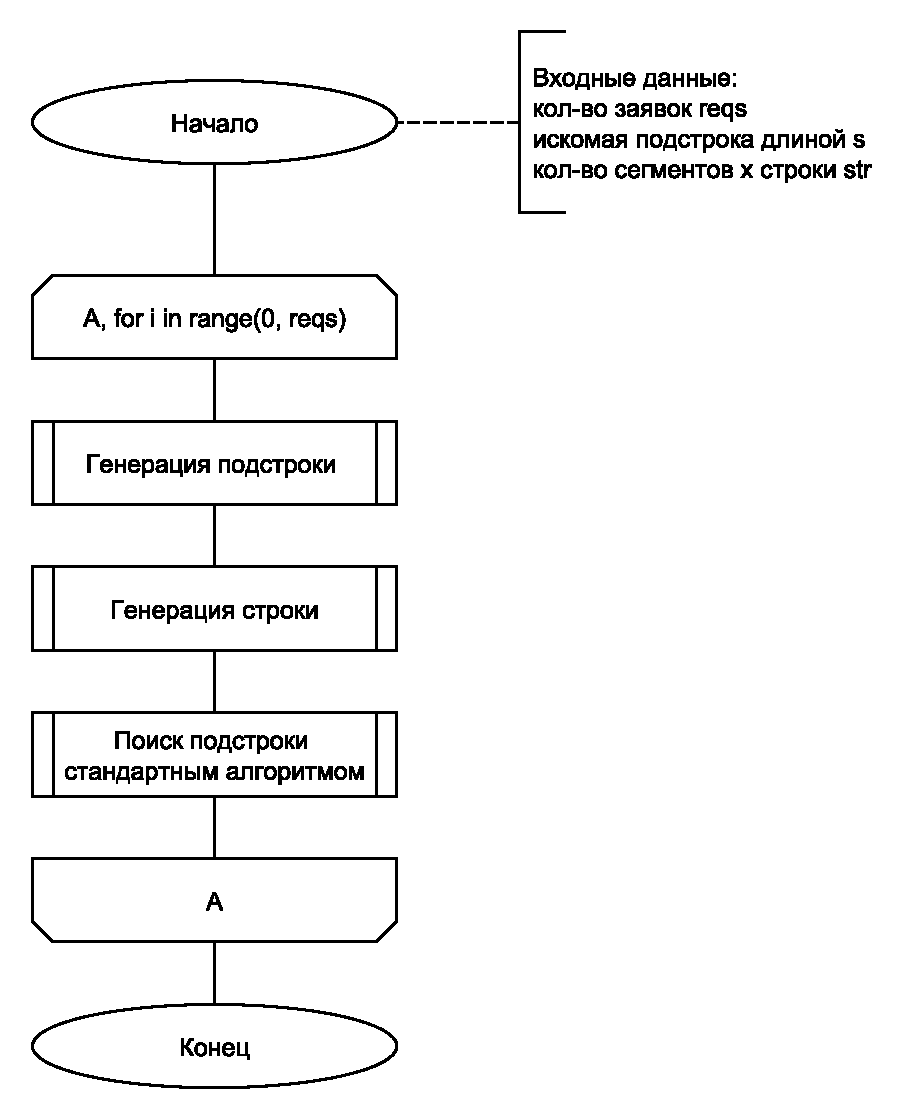
\includegraphics[width=0.7\linewidth]{images/linear}
	\caption[]{Последовательная реализация}
	\label{fig:linear}
\end{figure}

\newpage
На рисунке~\ref{fig:parallel} приведена реализация программы с двумя потоками.

\begin{figure}
	\centering
	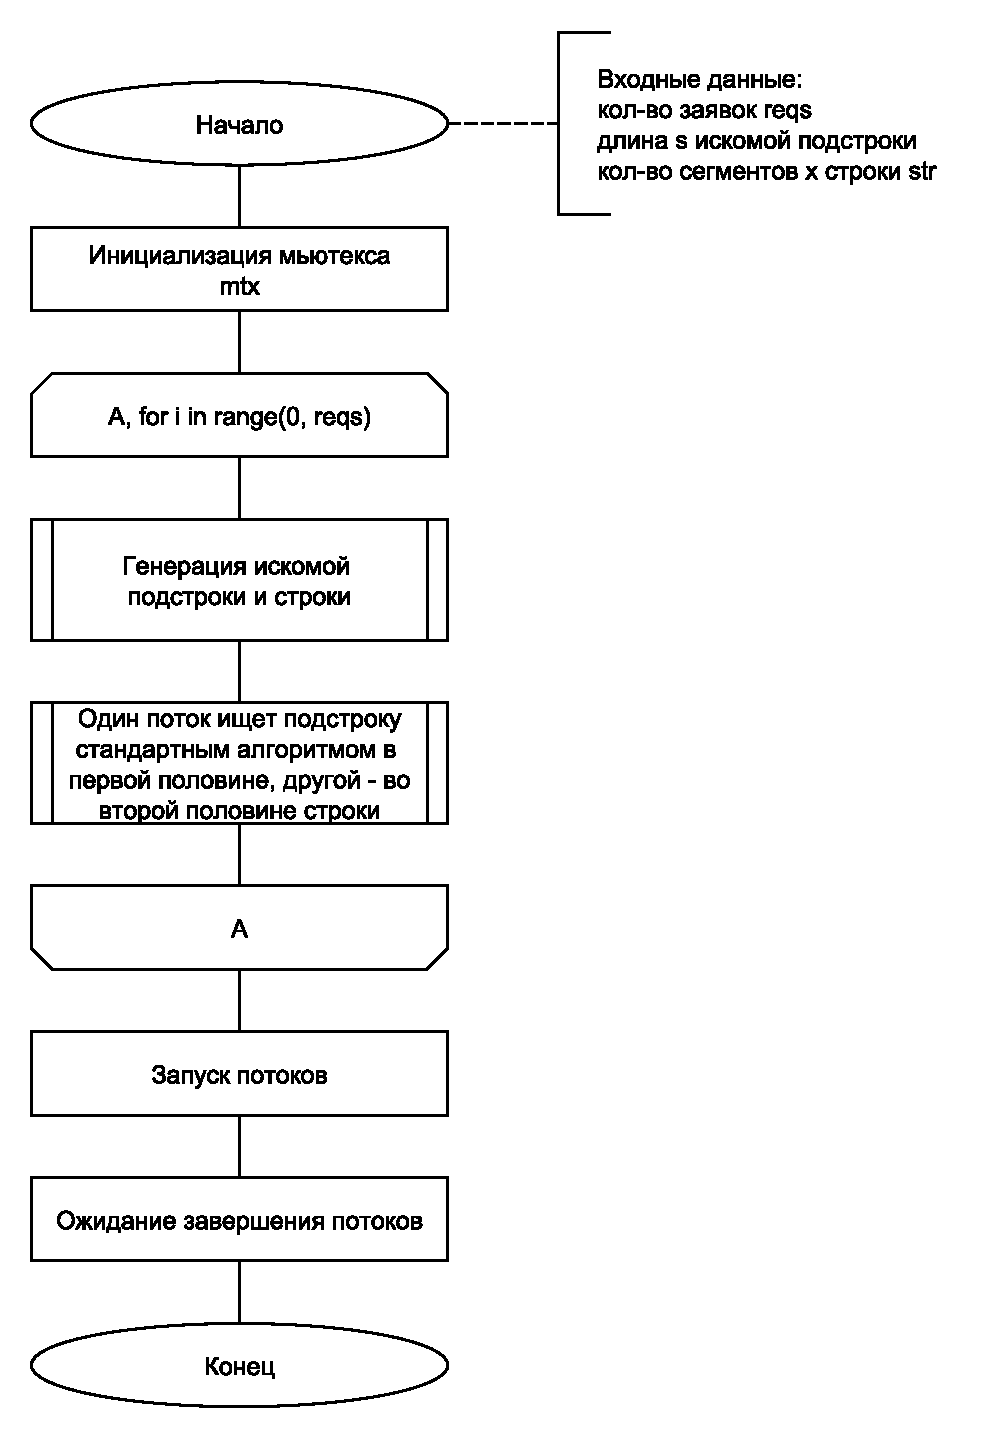
\includegraphics[width=0.7\linewidth]{images/parallel}
	\caption[]{Параллельная реализация}
	\label{fig:parallel}
\end{figure}

\newpage
При этом, функция записи лога на рисунке~\ref{fig:log} содержит критическую секцию, доступ к которой ограничивается мьютексом, который передается каждому потоку.

\begin{figure}
	\centering
	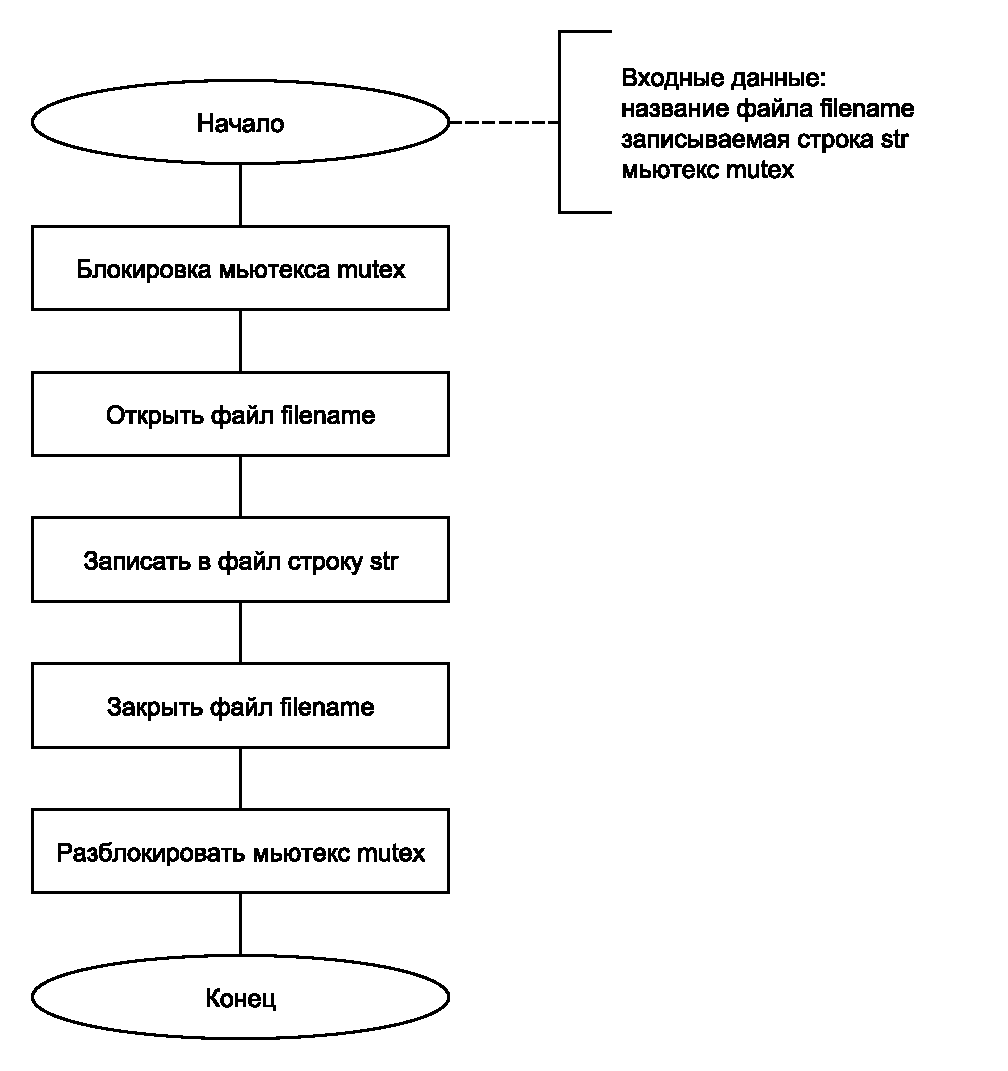
\includegraphics[width=0.7\linewidth]{images/log.pdf}
	\caption[]{Запись строки в файл}
	\label{fig:log}
\end{figure}